% !TEX encoding = UTF-8 Unicode
%!TEX root = main.tex
% !TEX spellcheck = en-US
%%=========================================

\chapter{Background}
\label{ch:background}

In this chapter a more in depth explanation of the different topics introduced in the introduction chapter is presented. These topics cover the required background knowledge for the project, which plays a central role in determining on what kind of development tool is to be implemented, how it is to be implemented, as well as showing what already exists of current solutions and tools.

Each topic is presented on its own, and how it relates and affects the choices of the development tool.


\section{Concurrency vs. Parallelism}
\label{sec:concurrency_vs_parallelism}

The notion of parallelism and concurrency in programs spawns from the limitations of sequential programs. All programming languages have different ways to express the structure and control flow of a program, but in the end all programs are transformed to machine code which the processor executes \textit{sequentially}. That means for a single processor, only one instruction is executed at a time\footnote{This implies the processor is single-core}. Concurrency however defines a program into multiple independent sequential programs, which in turn runs each sequential program in interleaving time periods. Even though only one instruction is executed at a time, this gives the impression that multiple sequential programs are advancing at the same time.

Parallelism in this sense refers to multiple programs running on multiple processors in parallel. This might look familiar to what concurrency described, but it is important to not confuse these two terms together. Concurrency only serves as an abstraction for parallelism in a program, allowing the programmer to pretend multiple sequential programs are executed in parallel. This abstraction would be valid for both single and multicore, while parallelism describes a condition which only happens on multicore. A more thorough and complete definition of concurrency and parallelism is described in \citet{benari2006}.

Concurrency and parallelism forms the very core of this project. Section \ref{sec:csp} explains what CSP is, and it forms its basis on concurrency. In Section \ref{sec:project_description} the project description of the CSP enabling development tool, so understanding the underlying concepts of concurrency is important to understand what CSP entails. Further on, multicore support was also mentioned as a motivation for the potential speedup, as a direct opportunity from the parallel nature in concurrent systems. Parallelism is directly tied to multicore, as both terms describe multiple programs executing simultaneously. 


\section{Threading Models}
\label{sec:threading_models}

As concurrency is is a superb tool for programmers to abstract parallelism in their program, the implementation details of this is equally as important for this project. There are different ways to implement this, but almost all concurrency models implement some sort of a threading mechanism. When talking about threading mechanisms on Operating Systems (OS), one usually talks about two kinds of threads: user- and kernel-threads. As the names may imply, these threads operate in either user- or kernel-space. Three main models explains the different combinations of the two threads: user-, kernel-, and hybrid-threading models. \citet{c++csp2} goes into further details on these models, and short summary is presented below from said article.

In short, the user-threading model implements a cooperative scheduled threading in user-space, and is called a M:1 threading model. This model is running M user-threads on a single kernel-thread, where everything from scheduling and context switching is happening unbeknownst to the kernel-thread. This means this threading mechanism is not visible to the OS, and avoids the overhead related to context switches in kernel-threads. However, blocking calls are a challenge, as a single blocking call will block all user-threads.

Kernel-threading model is often directly supported in OS kernels, and is called a 1:1 threading model. Each kernel-thread is scheduled by the OS onto the the systems processors. Scheduling is often implemented as preemptive, and due to kernel-threads residing in kernel-space gives context switches a much larger overhead than user-threading. Blocking calls are however not a problem. 

Hybrid-threading model combines the two models, and is called a M:N threading model. This model is running multiple kernel-threads, with each kernel-thread running multiple user-threads. Blocking calls is still a problem, but can be mitigated through dispatching a single kernel-thread for the block user-thread, and continue the rest of the scheduling on a new kernel-thread. 


\section{Memory Layout of C Programs}
\label{sec:memory_layout_c}

\FloatBarrier

The C programming language defines a memory layout of its programs. A total of 5 sections defines the memory layout.

\begin{enumerate}[topsep=0em,itemsep=-1em,partopsep=0.5em,parsep=1em]
    \item Text segment
    \item Initialized data segment
    \item Uninitialized data segment
    \item Stack
    \item Heap
\end{enumerate}

The text segment contains the executable code of instructions. The initialized data segment contains global and static variables that are initialized by the programmer. The uninitialized data segment contain all zero initialized or non\hyp{}initialized variables and data. The stack contains the program stack and stack frames, while the heap contains dynamic memory. The stack grows downwards, from higher to lower address, opposed to the heap which grows upwards, from lower to higher address. 

The unmapped segment is a precursor to the stack, containing command-line arguments and environment variables sent as program arguments. 

See Figure \ref{fig:c_memory_layout} for outline of the memory layout.

\begin{figure}[h!]
    \centering
    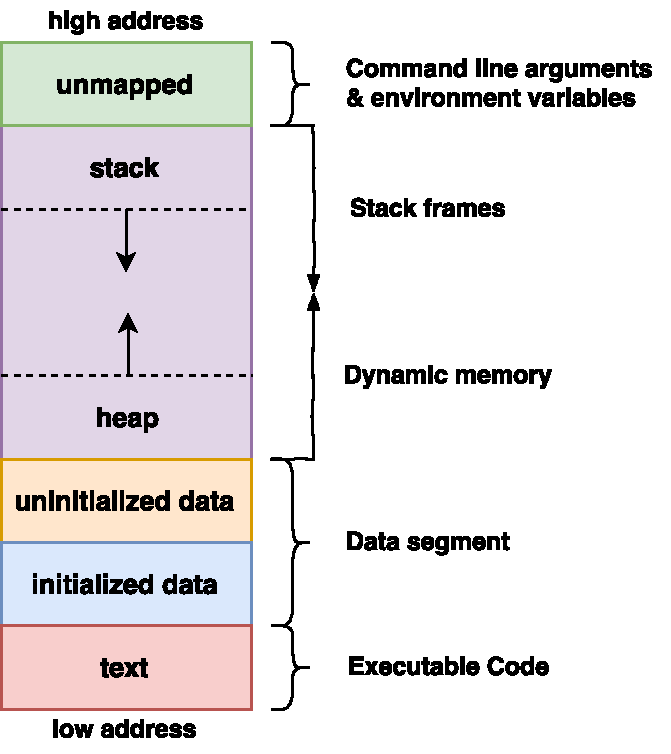
\includegraphics[width=0.5\linewidth]{fig/c_memory_layout}
    \caption{Memory layout of a C program}
    \label{fig:c_memory_layout}
\end{figure}

\FloatBarrier

\section{Stackful Coroutines}
\label{sec:stackful_coroutines}

Coroutines is a generalized subroutines within a program, used for non-preemptive multitasking. This allows a single\hyp{}threaded program to suspend and resume multiple executions, through predetermined scheduling points. There exists two types of coroutines implementations: stackful and stackless. As the name implies, stackful coroutines has each a corresponding stack which acts as the stack frame for that given coroutine. While for stackless coroutines, the main stack frame is used by all coroutines.

Resuming and suspending stackful coroutines involves storing and swapping contexts of coroutines. Each coroutine has a context which represents the execution state of a coroutine at a given time. This execution state can be seen as a snapshot of the processor registers of a given place in the code execution. Suspending a coroutine is a matter of storing the current execution state in memory, and replace the execution state with an another coroutine. Lastly, the program counter is replaced with resuming coroutine. This effectively suspends the initial coroutine, and resumes the other. 

Knowing what to store in execution states requires knowledge of the processor state, which is architecture dependent. This is why coroutine implementations often cause portability issues. The solution to this is looking at the calling convention for System V ABI \citep{systemvabi}, which is the convention almost all UNIX\hyp{}like architectures follow. 

Calling conventions describes how, on a low\hyp{}level, subroutines receive parameters from their caller and how they return their result. This usually describes on register level what registers must be preserved by the callee, and which must not. Knowing this, a context structure and a context switching procedure can be outlined. 

The context structure should contain the preserved registers, specified by the calling convention, and the program counter for a given coroutine. 


\section{Communicating Sequential Processes}
\label{sec:csp}

First introduced by Tony Hoare in 1978 \citep{csp}, Communicating Sequential Programming (CSP) aimed to make concurrency and parallelism a much more convenient tool for programmers. Even though CSP in itself is a mathematical formal language, the concepts and structuring it introduces is very applicable as a programming model. The core concept of CSP is a composition of concurrent sequential processes, which strictly communicate by message passing via channels.

Despite CSP being a great model for describing concurrent systems, it has not gained much mainstream traction within programming communities and industries. As detailed in \citet{benari2006}, concurrent programming introduces new challenges such as race conditions, deadlocks and fairness. These challenges can for many programmers be a hurdle to create correct concurrent programs, shown in \citet{ousterhour1996}. As a result of this they might end up opting in for other simpler programming models, and in turn miss out of CSP. 

This does not mean however that there does not exists CSP implementations. These implementations range from programmings languages which implements the CSP model (Section \ref{subsec:csp_prog_lang}), CSP libraries for more mainstream non-CSP programming languages (Section \ref{subsec:csp_prog_lib}), and CSP language compilers (Section \ref{subsec:csp_comp_runtime}).

The CSP implementations range in varying popularity and use, and below is a summary of the most notable entries which relates to this project presented.


\subsection{Programming Languages}
\label{subsec:csp_prog_lang}

Multiple programming languages implementing the CSP models in varying degree exists. Probably the most notable and truest implementation of the CSP model is occam. Other languages such as XC and Go is heavily influenced by the CSP model and occam. There exists other CSP languages such as Limbo \citep{limbo}, Joyce \citep{joyce}, and SuperPascal \citep{superpascal}, however occam, XC and Go seems to be the most influential and used languages to date\footnote{This is a highly subjective view, subjected on the popularity and relevance in the industry}. 


\subsubsection{Occam}
\label{sssec:occam}

Occam is a concurrent programming language which builds upon the CSP model. It was created by INMOS \citep{occam} and first appeared in 1983. Occam was initially developed as the native programming language for the Transputer, their microprocessor architecture highly specialized for real-time parallel computing \citep{transputer}. 

Occam was initially only developed for the Transputer, making it hardware locked and inaccessible for everyone not using the Transputer. However, occam proved to be quite express and useful for concurrent programming, which spurred multiple ports and compilers of occam to other open architectures. 

Sadly, occam never quite took off, and instead got its place in a niche market of real-time parallel computing with its highly specialized microprocessor Transputer. A decade almost went before the first portable occam compiler surfaced as SPoC \citep{spoc}, which made occam ``available'' for the public. This is only a speculation, but one can argue if INMOS had the wrong ambitions for this language, as their focus was more on the raw processing power on the Transputer rather than the expressive power in their language \citep{occam}. 

Whatever the reason was for occam's lack of popularity, occam definitely deserves more love than it has received by the general public. Its incredibly cool concepts and expressive power of concurrent systems should have its place in the mainstream programming industry, and with the onset of Go and its rise in popularity, it seems the mainstream programming industry might be mature enough for CSP.


\subsubsection{XC}
\label{sssec:xc}

XC is a concurrent programming language, which builds upon the concurrency and parallelism introduced in occam, and the syntax is based on C with new extensions and some minor restrictions. XC is targeted as the native programming language on the XCore processor architecture, created by XMOS \citep{xc}. XC first appeared in 2005.

XCore is a multi-core processor for embedded system, aimed at utilizing concurrency and parallelism natively. The only major implementation of XC is for the XCore architecture, making XC a hardware locked language such as occam was initially. 

Some of the interesting features XC introduces are expressive parallelism, communication between tasks through interfaces and channels, event handling on multiple guarded events, hardware support for timers and IO access, safe and unsafe memory access, and more.

Since there are no other major implementations of XC for other than XCore, it has more or less gained a niche market in embedded real-time parallel computing. XC achieves a lot with a great memory safety model, strict rules on communication, and good integration with its hardware, as well as not only focusing on raw performance, but also on determinism of execution time. 

\subsubsection{Go}
\label{sssec:go}

Go is a concurrent programming language, created and developed by Google \citep{golangintro}, and first appeared in 2009. Go does not build itself completely on the CSP model, but implements many features and ideas from CSP. This includes channels, parallel composition of asynchronous processes, and event handling on multiple channels with \texttt{select} \citep{golangspec}.

Go started as a desire of a modern concurrent language, which was both fast and scalable, and supported networking and multiprocessing. Go has since its initial launch in 2009 risen in popularity. As Go was not designed for a specific architecture, compared to occam and XC, has made Go quite popular in the networking industry. As the writing of this paper, Go ranks as the 13th most popular programming language on the TIOBE Index \citep{gopopularity}.

The popularity of Go has proven that the mainstream programming communities and industries are mature enough for a proper concurrency programming language. If other languages will finally follow after is only a matter of time.


\subsection{Programming Libraries}
\label{subsec:csp_prog_lib}

With the lack of concurrent programming languages, CSP libraries have been developed for existing sequential, imperative programming languages. This includes libraries such as JCSP \citep{jcsp}, C++CSP2 \citep{c++csp2}, PyCSP \citep{pycsp}, and CSP.NET \citep{cspnet}, however only JCSP and C++CSP2 will be summarized below as of relevance to this project.


\subsubsection{C++CSP2}
\label{sssec:c++csp2}

C++CSP2 \citep{c++csp2} is a concurrency library for C++. The original library C++CSP \citep{c++csp} provided the same features as C++CSP2, used however only user-threads for its concurrency. C++CSP2 aimed to redesign the implementation of the library into a many-to-many threading model, which would be more adequate for utilizing multi-core processors. 

Much of the implementation and design regarding the CSP features and constructs are detailed in \citet{c++csp}, while the details regarding the multi-core support of the concurrency model are in \citet{c++csp2}.

C++CSP2 provide CSP features such as processes, buffered/unbuffered typed one-direct\hyp{}ional channels, channel Poison for easily shutting down concurrent programs, time functions, alternative construct for expressing choice, barrier synchronization, and smart pointer Mobile to prevent aliasing. These features and more are explained in more detail in the documentation \citep{c++csp2doc}.


\subsubsection{JCSP}
\label{sssec:jcsp}

JCSP \citep{jcsp} is a concurrency library for Java. It offers the same features in C++CSP2 \citep{c++csp2}, building upon the CSP model. Compared to C++CSP2, JCSP focuses on more reliable and secure networking, and increases coding safety through promoting CSP specifiers to first-class entries. Other than that, they both provide a thorough CSP library. More information regarding the library and its features are found in the documentation \citep{jcspdoc}. 


\subsection{Compilers and Run-Time Environments}
\label{subsec:csp_comp_runtime}

As mentioned in Section \ref{subsec:csp_prog_lib}, some CSP libraries have been developed as a consequence on the lack of concurrent programming languages implementing the CSP model. Taking this further, portable compilers and run-time environments have been developed on already existing, unavailable CSP languages, namely occam. Below are the most influential and used compilers and run-time environments summarized. 


\subsubsection{SPoC}
\label{sssec:spoc}

The Southampton's Portable occam Compiler (SPoC) \citep{spoc} is a compiler for occam, making occam programs portable on industry-standard platforms. It achieves this by translating occam source code to ANSI-C, and then using a native C compiler on the generated output. Because of this, SPoC calls itself an occam-to-C translator. 

SPoC was the first major implementation of an occam compiler that was not for the Transputer processor architecture. This opened up the exploitation of the language, and proving occam's usefulness as a concurrent programming language.


\subsubsection{KRoC}
\label{sssec:kroc}

The Kent Retargetable occam Compiler (KRoC) \citep{kroc} is an emulator of the transputer, acting as a architectural mapping, or an emulator, rather than a compiler.

KRoC works by taking the transputer assembly from a compiled occam program and emulating the transputer hardware. This is achieved through emulating the transputer on a register-level, using the native registers of the targeted architecture. The SPARC architecture was the first retargetable architecture supported. 

Initially, the standard toolset occam compiler was used to generate the transputer assembly file, but proved that other occam compilers could be supplied. 


\subsubsection{CCSP}
\label{sssec:ccsp}

CCSP \citep{ccsp} is a portable run-time system that support both occam and C, enabling occam-like programming in C. It also supports KRoC occam system for desktop platforms. CCSP aims to fulfill the shortcomings of KRoC, such as support for C and making debugging useful.

Initially, CCSP only supported uniprocessors, but support for SMP\footnote{Symmetric MultiProcessing} was planned. 

FIXME